\documentclass{beamer}


\usepackage[frenchb]{babel}
\usepackage[T1]{fontenc}
\usepackage[utf8]{inputenc}
\usetheme{Warsaw}

\newcommand{\gr}{\textbf}
\newcommand{\info}[1]{\text{{\fontfamily{lmss}\selectfont #1}}}
\newcommand{\Mod}{\info{Mod}}
\newcommand{\Sen}{\info{Sen}}
\newcommand{\itemz}{\item[$\triangleright$]}
\newcommand{\il}{\textit}
\usepackage{stmaryrd}
\usepackage{tikz-cd} 
\usepackage{graphicx} % Allows including images
\usepackage{booktabs} % Allows the use of \toprule, \midrule and \bottomrule in tables

%----------------------------------------------------------------------------------------
%	TITLE PAGE
%----------------------------------------------------------------------------------------

\title[Morpho-logique]{Ultraproduits et généralisation du théorème de \L o\'s dans les institutions stratifiées}
\author{Alexandre Goy}
\institute[Parcours MP]
{
CentraleSupélec, Parcours Maths-Physique
}
\date{\today}

\begin{document}

\begin{frame}
\titlepage
\end{frame}

\section*{Introduction}

\begin{frame}
La logique est la base de l'informatique.
\begin{itemize}
\itemz Elle en est la base théorique : calculabilité, indécidabilité, classification des problèmes selon leur complexité.
\itemz La programmation est une activité logique : concevoir un programme, c'est prouver une proposition de façon constructive.
\end{itemize}
\pause
Problème d'informatique $\rightsquigarrow$ utilisation d'une logique existante ou définition d'une nouvelle logique dédiée à ce problème. \pause 
\begin{itemize}
\itemz \'Electronique : logique propositionnelle
\itemz Programmes standards : logique du premier ordre
\itemz Systèmes réactifs : logique modale temporelle
\end{itemize} \pause 
\textbf{Conséquence :} Il existe un très grand nombre de logiques.

\end{frame}

\begin{frame}
\frametitle{Plan de l'exposé}
\begin{itemize}
\itemz Présentation de trois logiques usuelles
\itemz Présentation de l'abstraction de ce qu'est une logique : les institutions \cite{Dia08}
\itemz Les problèmes des institutions ont mené à deux développements
\begin{itemize}
\itemz Les institutions stratifiées (prise en compte de la notion d'état) \cite{Aig07}
\itemz La morpho-logique (prise en compte de la structure des formules logiques) \cite{Aig17}
\end{itemize}
\end{itemize}
\end{frame}

\section{Logique}

\subsection{Trois logiques usuelles}

\begin{frame}
3 exemples de logiques usuelles
\begin{itemize}
\itemz Logique propositionnelle
\itemz Logique des prédicats du premier ordre
\itemz Logique modale
\end{itemize}
\end{frame}

\begin{frame}
\frametitle{Logique propositionnelle}
Les formules sont définies par induction.
\pause
\begin{itemize}
\itemz Formule atomiques : variables $p$, où $p \in \mathcal{P}$.
\pause
\itemz Si $\varphi$ et $\psi$ sont des formules alors
\pause
\begin{itemize}
\itemz $\varphi \wedge \psi$
\pause
\itemz $\varphi \vee \psi$
\pause
\itemz $\varphi \Rightarrow \psi$
\pause
\itemz $\neg \varphi$
\end{itemize}
sont des formules.
\end{itemize}
\pause
Quel sens donner à ces formules ? \\
Valuation $v : \mathcal{P} \to \{0,1\}$ + Tables de vérité
\pause
\begin{center}
\begin{tabular}{|c|c|c|c|c|c|}
  \hline
  $\varphi$ & $\psi$ & $\varphi \wedge \psi$ & $\varphi \vee \psi$ & $\varphi \Rightarrow \psi$ & $\neg \varphi$ \\
  \hline
  0 & 0 & 0 & 0 & 1 & 1 \\ 
  0 & 1 & 0 & 1 & 1 & 1 \\
  1 & 0 & 0 & 1 & 0 & 0 \\
  1 & 1 & 1 & 1 & 1 & 0 \\
  \hline
\end{tabular}
\end{center}
\end{frame}

\begin{frame}
\frametitle{Logique propositionnelle}
\textbf{Exemple.}\\
Un vol a été commis.\\
S'il a vérifié l'homogénéité de son butin, alors le voleur est un physicien. Si c'était un mathématicien, alors il n'a pas divisé par zéro. Quoi qu'il en soit, le voleur était un mathématicien ou un physicien. \pause
\begin{align*}
& p = \text{ "le voleur est un physicien" } \\
& m = \text{ "le voleur est un mathématicien" } \\
& h = \text{ "le voleur a vérifié l'homogénéité" } \\
& z = \text{ "le voleur a divisé par zéro" }
\end{align*}
\pause
\[ (h \Rightarrow p) \wedge (m \Rightarrow \neg z) \wedge (m \vee p) \]
\end{frame}

\begin{frame}
\frametitle{Logique des prédicats du premier ordre}
On se donne un langage, i.e., des ensembles de symboles \pause
\begin{itemize}
\itemz $\mathcal{C}$ symboles de constantes
\pause
\itemz $\mathcal{F}_n$ symboles de fonctions à $n$ variables
\pause
\itemz $\mathcal{R}_n$ symboles de relations à $n$ variables
\end{itemize}
\pause
Les formules sont définies par induction. \pause
\begin{itemize}
\itemz Formules atomiques : $R(t_1,...t_n)$ où les $t_i$ sont des termes (construits à partir de variables $x \in \mathcal{V}$, de $\mathcal{C}$, et de $\mathcal{F}_n, n \geq 0$)
\pause
\itemz $\varphi \wedge \psi$, $\varphi \vee \psi$, $\varphi \Rightarrow \psi$, $\neg \varphi$ sont des formules
\pause
\itemz $\forall x, \psi$ et $\exists x, \psi$ sont des formules (pour tout $x \in \mathcal{V}$)
\end{itemize}
\end{frame}

\begin{frame}
\frametitle{Logique des prédicats du premier ordre}
\textbf{Exemple.} Le langage des groupes.
\begin{itemize} 
\itemz $\mathcal{C} = \{ e \}$ élément neutre
\itemz $\mathcal{F}_2 = \{ * \}$ loi de groupe
\itemz $\mathcal{R}_2 = \{ = \}$ égalité
\end{itemize}
\pause
$\varphi : $ "Chaque élément du groupe a un inverse"
\pause
\[ \varphi : \forall g, \exists h, (g * h = e) \wedge (h * g = e) \]
\pause
Quel sens donner à ces formules ? \pause \\
Notion de \textit{modèle}. \pause
Par exemple, $\mathbb{Z}$ est un modèle pour le langage des groupes : 
\[ e \mapsto 0_\mathbb{Z} \]
\[ * \mapsto +_\mathbb{Z} \]
\[ = \mapsto =_\mathbb{Z} \]
On notera $\mathbb{Z} \models \varphi$ ou encore $\mathbb{N} \not\models \varphi$.

\end{frame}

\begin{frame}
\frametitle{Logique modale}
\begin{itemize}
\itemz Formules atomiques : $p \in \mathcal{V}$ \pause
\itemz $\varphi \wedge \psi$, $\varphi \vee \psi$, $\varphi \Rightarrow \psi$, $\neg \varphi$ \pause
\itemz $\square \varphi$ (il est nécessaire que $\varphi$ soit vraie) \pause
\itemz $\Diamond \varphi$ (il est possible que $\varphi$ soit vraie) \pause
\end{itemize}
\pause
Quel sens donner à ces formules ? \pause \\ $\longrightarrow$ Modèles de Kripke (mondes possibles). \pause \\~\\
\textbf{Exemple.} $\varphi$ = "Napoléon est vivant" \pause
\begin{itemize}
\itemz $\varphi$ \pause est vraie si l'on se situe entre 1769 et 1821 \pause
\itemz $\square \varphi$ \pause est fausse ; il n'est pas nécessaire que Napoléon soit vivant, la preuve, il ne l'est plus aujourd'hui \pause
\itemz $\Diamond \varphi$ \pause est vraie : il est possible que Napoléon soit vivant, la preuve, il l'a déjà été \pause
\end{itemize}
On a besoin d'une notion \textit{d'état} du système.

\end{frame}

\subsection{Une structuration commune}

\begin{frame}
Toutes ces logiques (et les autres ont la même structure) :
\begin{itemize}
\itemz Une \textbf{signature},
\itemz Des \textbf{formules},
\itemz Des \textbf{modèles},
\itemz Une \textbf{relation de satisfaction} $\models$.
\end{itemize}
\pause
\begin{center}
\begin{tabular}{|c|c|c|c|c|c|}
  \hline
  & Logique propositionnelle \\
  \hline
  Signature & $\mathcal{P}$  \\ 
  Formules & Par induction avec $\wedge,\vee,\Rightarrow,\neg$ \\
  Modèles & Valuations $v : \mathcal{P} \to \{ 0 , 1 \}$  \\
  Satisfaction & Tables de vérité \\
  \hline
\end{tabular}
\end{center}
\end{frame}

\subsection{Institutions (stratifiées)}

\begin{frame}[fragile]
\begin{definition}[Catégorie]
Une catégorie $\textbf{C}$ est composée
\begin{itemize}
\itemz D'objets $A,B,C$...
\itemz De morphismes entre les objets $f : A \to B$, $g : B \to C$...
\itemz D'une loi de composition notée $g \circ f$.
\itemz Pour chaque objet $A$, d'un élément neutre $id_A : A \to A$.
\end{itemize}
\end{definition} \pause 
\begin{center}
\begin{tikzcd}
\cdot & \cdot \arrow[r] & \cdot \arrow[d] \\
\cdot \arrow[u] \arrow[ur] & \cdot \arrow[l] \arrow[u] & \cdot \arrow[ul]
\end{tikzcd}
\end{center}
\pause
\gr{Exemples.} La catégorie des ensembles $\textbf{Set}$.\\ La catégorie des catégories $\textbf{Cat}$. 
\end{frame}

\begin{frame}[fragile]
\begin{definition}[Foncteur]
Soit $\gr{C}$, $\gr{D}$ deux catégories. Un foncteur $F : \gr{C} \to \gr{D}$ associe 
\begin{itemize}
\item \`A chaque objet $A$ de $\gr{C}$, un objet $F(A)$ de $\gr{D}$.
\item \`A chaque morphisme $f : A \to B$ de $\gr{C}$, un morphisme $F(f) : F(A) \to F(B)$. 
\end{itemize}
De plus, $F(g \circ f) = F(g) \circ F(f)$ ($F$ est covariant) ou $F(g \circ f) = F(f) \circ F(g)$ ($F$ est contravariant). 
\end{definition}
\pause
\begin{center}
\begin{tikzpicture}[baseline= (a).base]
\node[scale=0.7] (a) at (0,0){

\begin{tikzcd}
\cdot \arrow[ddrr,""{name=1}] \arrow[dd,""{name=2}] \arrow[drrrr,dashed] & & \textbf{C} & & & &  \\
& & & & |[alias=U]| \cdot \arrow[ddrr,""{name=1'}] \arrow[dd,""{name=2'}] & & \textbf{D} \\
\cdot \arrow[rr,""{name=3}] \arrow[drrrr,dashed] & & \cdot \arrow[drrrr,dashed] & & & & \\
& & & & |[alias=D]| \cdot \arrow[rr,""{name=3'}] & & |[alias=R]| \cdot 

\arrow[from=1, to=1', dotted]
\arrow[from=3, to=3', dotted]
\arrow[from=U, to=D, crossing over]
\arrow[from=2, to=2', dotted]

\end{tikzcd}
};
\end{tikzpicture}
\end{center}

\end{frame}

\begin{frame}

\begin{definition}[Institution]
Une institution $\mathcal{I}$ est composée de
\begin{itemize}
\itemz Signature : une catégorie $\textbf{Sig}$
\itemz Formules : un foncteur $\Sen : \textbf{Sig} \to \textbf{Set}$
\itemz Modèles : un foncteur (contravariant) $\Mod : \textbf{Sig} \to \textbf{Cat}$
\itemz Satisfaction : pour toute signature $\Sigma \in \textbf{Sig}$, une relation $\models_\Sigma$ entre $\Mod(\Sigma)$ et $\Sen(\Sigma)$.
\end{itemize}
\end{definition}

\end{frame}

\begin{frame}
Comment prendre en compte la notion d'état ? \pause
\begin{definition}[Stratification]
Une institution \textit{stratifiée} est une institution munie d'une stratification, i.e., d'une famille de foncteurs $\llbracket - \rrbracket_\Sigma : \Mod(\Sigma) \to \gr{Set}$.
\end{definition}
$\llbracket M \rrbracket_\Sigma$ est l'ensemble des états de $M$. \\
\pause
La relation de satisfaction $\models_\Sigma$ est paramétrée par les états : $\models_\Sigma^\eta$.\\
$\longrightarrow$ Une formule peut être vraie ou fausse en fonction de l'état du système. \\~\\
On peut définir, par exemple, des topologies sur les ensembles d'états (cf logique $\textbf{TMPL}$ dans le rapport).
\end{frame}

\section{Vers la morpho-logique}

\subsection{Motivation}
\begin{frame}
\gr{Problème} : $\Sen : \gr{Sig} \to \gr{Set}$, mais en pratique les formules sont toujours définies par induction.\\~\\ \pause
Comment définir nos formules par induction, mais en les laissant abstraites ? \pause \\~\\
Logique du premier ordre = logique propositionnelle + $\forall$ + $\exists$\\
Logique modale = logique propositionnelle + $\square$ + $\Diamond$\\ \pause
\begin{align*}
& \neg \forall x, \varphi \leftrightarrow \exists x, \neg \varphi \\
& \forall x, (\varphi \wedge \psi) \leftrightarrow (\forall x, \varphi) \wedge (\forall x, \psi) \\
& \exists x, (\varphi \vee \psi) \leftrightarrow (\exists x, \varphi) \vee (\exists x, \psi)
\end{align*} \pause
$\square$ et $\Diamond$ vérifient les mêmes propriétés de dualité
\end{frame}

\subsection{Morphologie mathématique}

\begin{frame}
Addition de Minkowski dans $\mathbb{R}^n$ et dilatation :
\begin{align*} & A \oplus B = \{ a + b \mid a \in A, b \in B \} &
 & D : X \mapsto X \oplus B
\end{align*}
\pause
Soustraction de Minkowski dans $\mathbb{R}^n$ et érosion : 
\begin{align*} & A \ominus B = \{ a \mid \forall b \in B , a + b \in A \}   & & E : X \mapsto X \ominus B
\end{align*}
\pause
\begin{center}
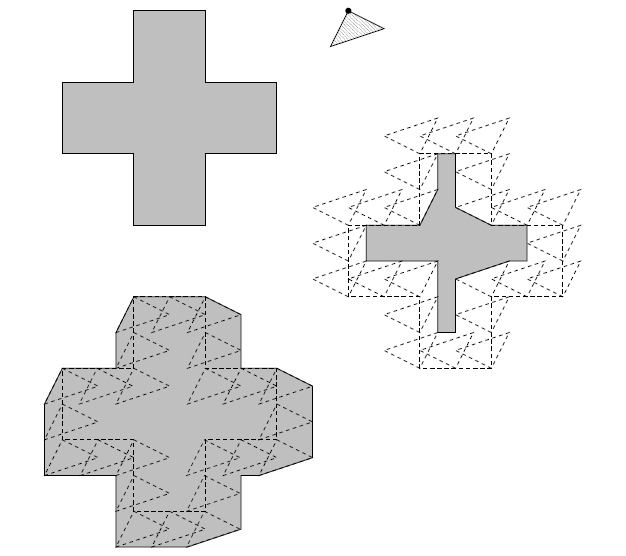
\includegraphics[scale=0.3]{erodil.png}
\end{center}
\end{frame}

\begin{frame}
Propriétés de dualité :
\begin{align*}
& ~^{c} E(X) = D(~^{c} X) \\
& E(X \cap Y) = E(X) \cap E(Y) \\
& D(X \cup Y) = D(X) \cup D(Y)
\end{align*} \pause
\begin{align*}
& \neg \forall x, \varphi \leftrightarrow \exists x, \neg \varphi \\
& \forall x, (\varphi \wedge \psi) \leftrightarrow (\forall x, \varphi) \wedge (\forall x, \psi) \\
& \exists x, (\varphi \vee \psi) \leftrightarrow (\exists x, \varphi) \vee (\exists x, \psi)
\end{align*} 
\textbf{Idée :} Prendre une classe d'opérateurs duaux abstraits $(E_i)_{i\in I}$ et $(D_i)_{i\in I}$ afin de modéliser n'importe quels nouveaux opérateurs logiques duaux tels que $\forall, \exists$ ou $\square, \Diamond$.
\end{frame}

\subsection{Morpho-logique}

\begin{frame}
\begin{center}
\begin{tabular}{|l|c|c|}
  \hline
   & \gr{Formules} \\
  \hline
  \il{Institutions} & Abstraites \\
  \hline
  \il{Morpho-logique} & $\neg,\wedge,\vee,\Rightarrow,(E_i)_{i\in I},(D_i)_{i\in I}$ \\
  \hline
\end{tabular}
\end{center}
\end{frame}

\begin{frame}
Exemple : le théorème de \L o\'s. \\
On peut le prouver avec une extrême lourdeur dans les institutions en général, mais sa preuve classique est par essence une induction sur les formules. C'est un bon crash-test pour notre théorie.
\begin{theorem}[\L o\'s]
Soit $I$ un ensemble et $\mathcal{U}$ un ultrafiltre sur $I$. Alors pour toute formule $\varphi = \varphi(x_1,...,x_n)$, pour tous $a_1,...,a_n \in \prod_{i\in I} M_i$, on a l'équivalence
\begin{align*}
 \prod_{i\in I} \mathcal{M}_i / \mathcal{U} \models \varphi(\pi(a_1),...,\pi(a_n)) \Longleftrightarrow ||\varphi(a_1,...,a_n)|| \in \mathcal{U}
\end{align*}
\end{theorem}
\end{frame}

\begin{frame}
\frametitle{References}
\footnotesize{
\begin{thebibliography}{99}
\bibitem[Aig17]{Aig17} Marc Aiguier, Isabelle Bloch (2017)
\newblock Dual Logic Concepts based on Mathematical Morphology in Stratified Institutions: Applications to Spatial Reasoning
\newblock \emph{CoRR} abs/1710.05661.

\bibitem[Aig07]{Aig07} Marc Aiguier, Răzvan Diaconescu (2007)
\newblock Stratified institutions and elementary homomorphisms
\newblock \emph{Information Processing Letters} 103(1), 5 --13.

\bibitem[Dia08]{Dia08} Răzvan Diaconescu (2008)
\newblock Institution-independent Model Theory
\newblock Birkhäuser Basel, 1st edition.

\end{thebibliography}
}
\end{frame}

%------------------------------------------------

\begin{frame}
\Huge{\centerline{Merci de votre attention}}
\end{frame}

%----------------------------------------------------------------------------------------

\end{document} 